\documentclass[12pt]{article}
\usepackage{amsmath}
\usepackage{graphicx}
\usepackage{listings}
\usepackage{verbatim}
\def\pp{\par\noindent}
\newcommand{\problem}[1]{\bigskip\pp\textbf{Part #1}\smallskip}
\renewcommand{\part}[1]{\smallskip\pp\textbf{#1)}\indent}
\newcommand{\given}{$\vert$~}
\newcommand{\prob}{\text{Pr}}
\begin{document}
\lstset{basicstyle=\small,language=Python,tabsize=2}
\centerline{CSE 544 - Final Project}
\centerline{Andrew Burford 112251367}
\centerline{Daniel Billmann 114715276}
\centerline{Efthimios Vlahos 110540896}

\problem{1}
\par We used pandas to read in the csv data and store it in a pandas
DataFrame object. Data was cleaned and outliers removed independently for each column of
data we are interested in. i.e. the daily cases in a specific state
was cleaned separately from the daily cases in a different state.
There were no empty rows within the CSV data we had to worry about.
While decumulatizing the rows, we noticed an issue in the cumulative
deaths data within MA:
\pp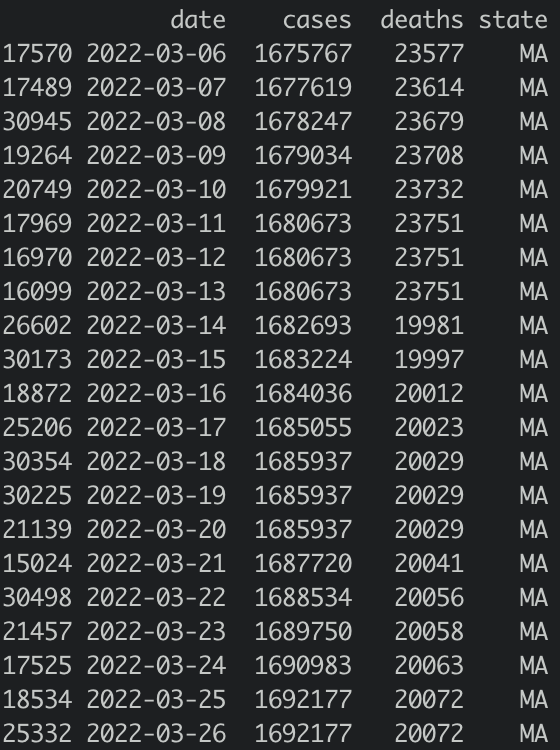
\includegraphics[scale=0.5]{cumulative_error.png}
\par You can see that on March 14th, 2022, the cumulative total drops.
This results in a negative number of deaths for this day, but it ends
up not mattering because this data point is dropped after applying
Tukey's rule. Here is the results of our cleaning script:
\verbatiminput{cleaning.log}
It is also worth noting that since we are taking the difference
between cumulative totals each day, we do not have data for the first
day in the data set so we always drop this day.
\problem{2}
\part{a}
\verbatiminput{part_a.log}
\par With regard to the validity of these tests, the one sample
t-tests are not valid for testing the hypothesis that the mean \# of
cases or deaths in February 2021 is different from the mean in March
2021 since they ignore the variance in the data in February. They
could only test the null hypothesis that the mean \# of cases/deaths in
March 2021 is equal to a specific value. For the 1
sample Wald's test, the test is just about applicable to test this
other hypothesis since we are using an asymptotically normal estimator
and our data set size is either very close to or just above 30, when
asymptotic normality kicks in. For 1 sample t-test, again this test is
applicable to the other hypothesis because n is just about equal to 30
so it does not matter whether the underlying data is normally
distributed. For the 1 sample z-test, we are using the much larger
data set of \#cases/deaths for the entire date range in the data set,
so this is a good way of getting an accurate estimate of population
standard deviation. This means the z-test is valid for testing this
other hypothesis as well. The 2 sample t-test is also essentially
valid since 28 is very close to 30 for the February sample even if the
underlying data is not normal, so the variance of the difference in
means will be approximately normal. The 2 sample Wald's test is valid
for the same reason. Both 2 sample tests apply to testing the null
hypothesis of equality of means between the two months.
\part{b}
\verbatiminput{part_b.log}
\part{c}
\verbatiminput{part_c.log}
\pp\includegraphics[scale=1]{2c.pdf}
\part{d}
\verbatiminput{part_d.log}
\part{e}
\par Some of the days in this date range had outliers in one state but
not the other. Since this is a paired t-test, we throw out any days
with an outlier in either state. This results in less than 30 days of
data.
\verbatiminput{part_e.log}
\par In both cases, we reject the null hypothesis under alpha = 0.5 in
favor of the alternative hypothesis that the number of vaccines
administered each day is different in MA than in MS. The positive t
statistics tell us that on average MA distributed more vaccines each
day. The largest reason for this is likely that there are simply more
people living in MA than in MS. MA has a population of about 6.9
million while MS is about 2.9 million.

\bigskip\pp\textbf{Exploratory Task}\smallskip
\pp Test 1
\par For this test we propose the null hypothesis that there is no
correlation between the number of daily COVID cases and the number of
daily gun deaths in the US.
\begin{verbatim}
Pearson Correlation for violent gun injuries and COVID cases.
With a rho value of 0.0009855083539563095, we do not reject the null
hypothesis that gun violence and the COVID-19 pandemic are correlated.

Pearson Correlation for violent gun deaths and COVID cases.
With a rho value of 0.0016163729398155522, we do not reject the null
hypothesis that gun violence and the COVID-19 pandemic are correlated.
\end{verbatim}

\pp Test 2
\par For this test, we consider the indicator variable that is equal
to 1 when more people in the US died of gun shots than people in NY
died of COVID and 0 otherwise. We propose the null hypothesis that the day of the
week is independent from this indicator. i.e. Whether or not gun shots in
the US killed my people than COVID did in NY is independent of the day
of the week.

\pp Test 3
\par For this test, we consider two variables: the percentage of gun
incidents (\# gun deaths + \# gun injuries) each day that are fatal, and
the percentage of COVID vaccines given to people in the US who are 65
and older. We test whether these two variables come from the same
distribution using a K-S test.

%\problem{1}
%\part{a} 
%\pp\includegraphics[scale=0.2]{1a}
%\begin{lstlisting}
%\end{lstlisting}

\end{document}
% vim:textwidth=70
